\chapter{Methodology}
\label{ch:methodology}

\section{The Classification Pipeline}

This thesis treats early-warning detection as a supervised time series classification (TSC) problem: train a classifier to recognise the shape of an approaching bifurcation, rather than compute one fixed statistic like variance or autocorrelation by hand.

\subsection{The Pipeline, Stage by Stage}

Figure~\ref{fig:pipeline} lays out the full pipeline end to end, and every box in it is defined precisely somewhere in this chapter. Two data sources -- \citet{bury2021}'s synthetic SDE corpus and the PANGAEA cores (Chapter~\ref{ch:data}) -- feed into one shared preprocessing step that treats both the same way, regardless of source: windowed by position, normalized by mean absolute value, never interpolated onto a uniform time grid. From there the pipeline splits by \emph{model family}, not by data source -- a synthetic example and a real one go through the same fork -- into a 5-channel path for the classical models and a 1-channel path for the deep-learning models. The two paths converge again at inference, and every one of the 29 models produces the same shape of output: a probability for each of the four classes. What happens to that output next depends on which data source it came from, which is the figure's last split: a synthetic test example has a true label, so it is scored with one-vs-rest macro AUC; a real PANGAEA segment does not, so only the narrower question of whether a transition was detected at all can be scored, against AR(1) null surrogates. Section~\ref{sec:evaluation_metrics} gives both metrics exactly.

\begin{figure}[htbp]
\centering
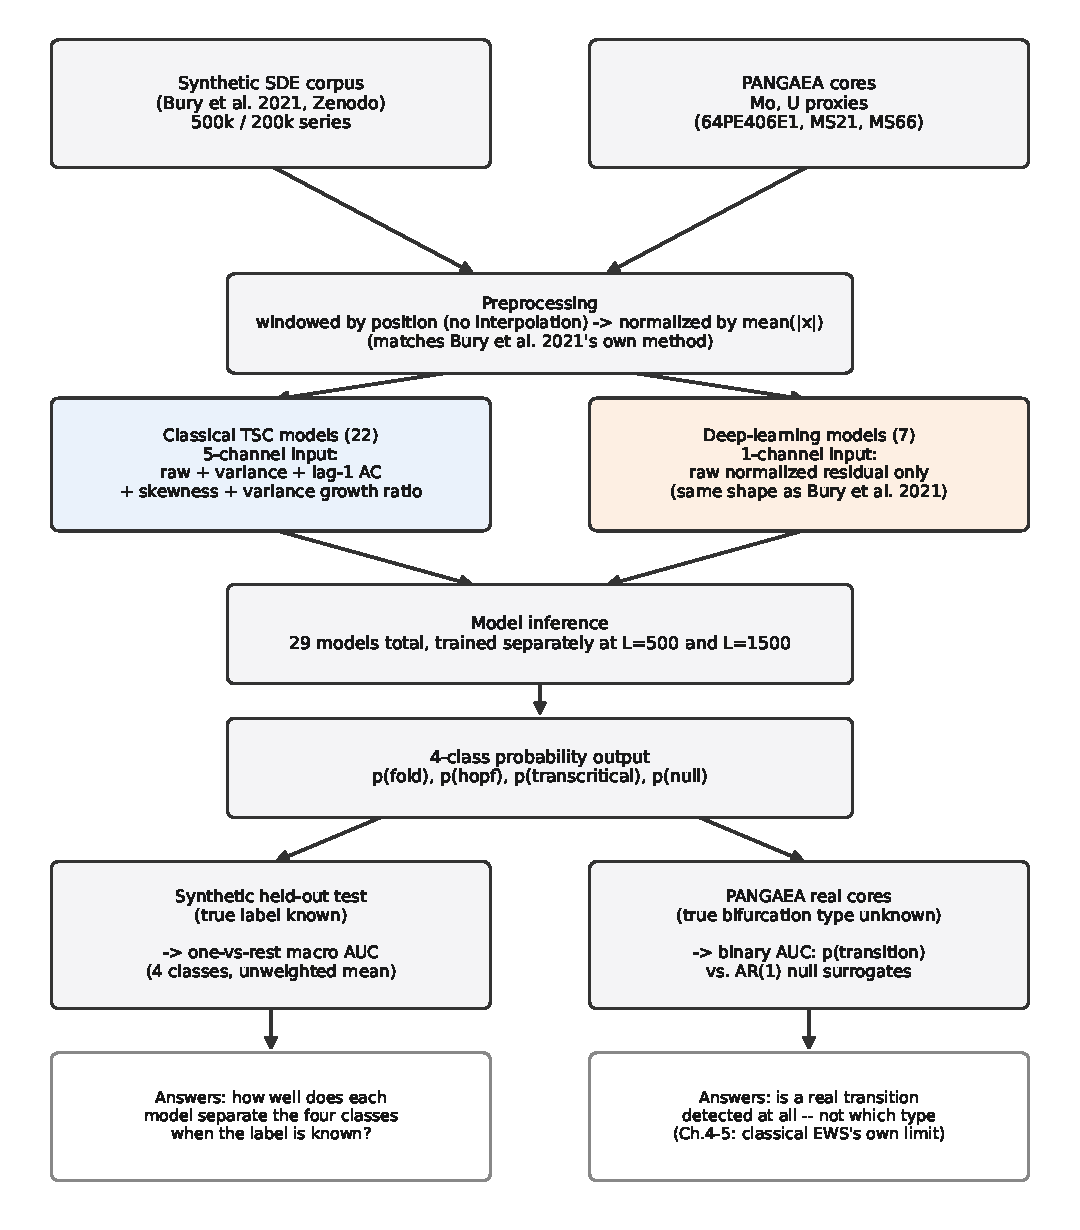
\includegraphics[width=0.85\textwidth]{figures/fig6_pipeline.pdf}
\caption{The full classification pipeline, from raw data to evaluated result. Every stage and every number shown here is defined precisely in the text that follows and cross-referenced to Chapter~\ref{ch:data}.}
\label{fig:pipeline}
\end{figure}

\begin{enumerate}
    \item \textbf{Data ingestion and preprocessing.} Raw series -- synthetic SDE output or empirical PANGAEA proxies (Mo, U) -- enter as 1D arrays. Chapter~\ref{ch:data}, Section~\ref{sec:preprocessing} describes the real preprocessing steps: samples are windowed by position, not resampled onto a uniform time grid, and every window is normalized by dividing by its own mean absolute value (matching \citet{bury2021}'s own method), not by a Z-score.
    \item \textbf{Feature engineering (classical models only).} The 22 classical TSC models have each normalized window expanded from one raw channel into five: the raw residual, rolling variance, rolling lag-1 autocorrelation, rolling skewness, and the variance growth ratio (Chapter~\ref{ch:data}, Section~\ref{sec:feature_engineering}). The 7 deep-learning models skip this step entirely and read the single normalized channel directly, the same shape \citet{bury2021}'s own classifier reads.
    \item \textbf{Model inference.} Each series -- 5-channel for a classical model, 1-channel for a deep-learning model -- is passed through one of the models described in this chapter.
    \item \textbf{Probabilistic output.} Every model, deep-learning or classical, exposes the same \texttt{predict\_proba()} method (confirmed directly in every \texttt{models/*.py} file), so the rest of the pipeline never has to know which kind of model it is talking to, or whether the input is synthetic or a real PANGAEA segment. For the deep-learning models this is a softmax over the final linear layer's logits (\texttt{torch.softmax}, e.g.\ \texttt{models/lstm.py}, \texttt{models/cnn\_lstm.py}). For a classical model it either delegates directly to the underlying aeon/scikit-learn classifier's own \texttt{predict\_proba} (most of the roster), or, for the ridge-regression-backed kernel classifiers (the ROCKET family) that only produce a raw decision score, applies the same softmax transform by hand to the \texttt{decision\_function} output (\texttt{models/tsc.py}) -- the "equivalent probability estimate" referenced in Section~\ref{sec:evaluation_metrics}.
    \item \textbf{Evaluation, split by data source.} This same \texttt{predict\_proba()} call -- including the ridge-regression classifiers' hand-computed softmax -- is what produces the output scored in both branches below on PANGAEA data as much as on synthetic data; only the scoring differs, not how the probability itself is obtained. The synthetic held-out test split has a known label, so every model's output there is scored by one-vs-rest macro AUC across the four classes. The real PANGAEA segments do not have a known bifurcation type, so their output -- from that same call, run on the real cores instead -- is scored only as a binary detection question, $p(\text{transition})$ against AR(1) null surrogates, which is the one question the real data can actually answer (Section~\ref{sec:evaluation_metrics}).

For a rougher, descriptive summary of the same output, this thesis also computes a favoured-class frequency, the same convention \citet{bury2021} use for their own Figure 2, whose insets report "the frequency of the favored DL probability among the forced trajectories" for each class: at each rolling-window position, the favoured class is simply $\arg\max$ over the four predicted probabilities (fold, hopf, transcritical, null), and the frequency reported for each class is the count of windows where it was the argmax, divided by the total number of windows in whatever group is being summarised -- a hard, winner-take-all count rather than an average of the raw probabilities, chosen specifically to match Bury et al.'s own convention rather than introduce a different one. Pooled this way across every model, sequence length, core, sapropel, and element in the corrected Mo/U dataset (25{,}960 forced-window predictions from 649 (model, dataset, core, sapropel, element) records), the favoured class splits 28.5\% fold, 37.4\% hopf, 14.6\% transcritical, and 19.5\% null. This is a raw description of the pipeline's output, not a filtered or weighted result -- it includes every model regardless of how well it performs on the labeled synthetic data, so it should not be read as a finding about which bifurcation type is correct; Chapter~\ref{ch:results} restricts to the trustworthy model subset and reports that properly, using the same argmax convention throughout.
\end{enumerate}

\subsection{Supervised Learning Framing}

The learning task is to approximate a function $f: \mathcal{X} \rightarrow \mathcal{Y}$, where $\mathcal{X}$ is the space of input windows of fixed length $L$ ($L=500$ or $L=1500$; both are used, Chapter~\ref{ch:data}) -- 5 channels wide for the classical models, 1 channel wide for the deep-learning models (previous subsection) -- and $\mathcal{Y} = \{0,1,2,3\}$ is the class label:

\begin{itemize}
    \item $y=0$: Fold bifurcation
    \item $y=1$: Hopf bifurcation
    \item $y=2$: Transcritical bifurcation
    \item $y=3$: Null (no transition)
\end{itemize}

(This ordering matches \texttt{src/constants.py}, the single source of truth for class indices used throughout the actual pipeline -- it is fold, hopf, transcritical, null, not the fold/transcritical/hopf/null order used earlier in this chapter's prose for readability. The index order matters for anyone reading the code directly, so it is stated precisely here.)

\subsection{Training, Validation, and Test Split}

The synthetic dataset's train/validation/test split is Bury et al.'s own, not one this thesis computes: their released \texttt{groups.csv} (Chapter~\ref{ch:data}) assigns every sequence a fixed \texttt{dataset\_ID} of 1 (train), 2 (val), or 3 (test), and \texttt{src/preprocess\_bury\_data.py} reads that column directly rather than performing any split itself. Counting each saved split file confirms the result is 95\% training, 4\% validation, 1\% test at both sequence lengths (475{,}000/20{,}000/5{,}000 of 500{,}000 series at $L=500$; 190{,}000/8{,}000/2{,}000 of 200{,}000 at $L=1500$) -- the same proportions recorded in \texttt{config.yaml}'s \texttt{train\_frac: 0.95, val\_frac: 0.04, test\_frac: 0.01} fields, though those fields are descriptive only: no code in this pipeline reads them to perform a split. This is a straightforward held-out split, not $K$-fold cross-validation -- no rotation of which examples are used for validation is performed. The validation split is used for early stopping and learning-rate scheduling during training (Section~\ref{sec:hyperparameters}); the test split gives one held-out synthetic accuracy number per model, reported in the results. After training, every model's weights are frozen before it is ever run on the real PANGAEA cores (Chapter~\ref{ch:data}, Section~\ref{sec:dual_dataset}).

\section{Deep Learning Architectures}
\label{sec:dl_architectures}

Seven deep-learning architectures are benchmarked. Three (LSTM, CNN-LSTM, InceptionTime) are explained in depth below since they represent the three broad design families in the roster (pure recurrence, hybrid, multi-scale convolution); the remaining four (ResNet, TCN, RNN-FCN, PatchTST) are newer additions to the roster this thesis contributes, each reproducing a specific published architecture as closely as PyTorch allows, verified layer-by-layer against a reference implementation (documented in full in \texttt{ARCHITECTURE\_COMPARISON.md} in the project repository).

\subsection{LSTM Baseline}

The LSTM baseline in this roster is not \citet{bury2021}'s architecture -- their own classifier is the CNN-LSTM hybrid described next. It instead follows \citet{ma2025sdml}: a dense layer from the raw input to an LSTM layer of 128 units, a dropout layer (rate 0.5), a second LSTM layer, a second dropout layer, a dense layer of 128 units with a ReLU activation, and a final dense layer to the class outputs -- confirmed against both the paper's own architecture description and this thesis's implementation (\texttt{models/lstm.py}). \citet{ma2025sdml} test this same architecture, alongside an SVM, a CNN, and a Multi-Head CNN, on the same three Mediterranean anoxia cores this thesis uses (Chapter~\ref{ch:data}), picking whichever classifier scored best per core -- the LSTM was their best performer specifically for core 64PE406E1 (F1 = 0.99). Their version outputs two classes (transition vs. no transition), trained with binary cross-entropy and the Adam optimizer; this thesis reuses the same architecture for its own four-class task.

An LSTM (Long Short-Term Memory network) is a recurrent architecture built to avoid the vanishing-gradient problem that affects simpler recurrent networks on long sequences, using an internal memory cell regulated by a forget gate, an input gate, and an output gate. Applied to a long, noisy series, a plain LSTM still has to process every point sequentially through that one memory cell, which can make it harder to keep track of a slow-moving signal buried in high-frequency noise.

\subsection{Convolutional Neural Network -- Long Short-Term Memory (CNN-LSTM)}

The CNN-LSTM hybrid is \citet{bury2021}'s own architecture, not an original one: it separates local feature extraction from long-range memory, so a convolutional layer first extracts local patterns (a short variance spike, a local autocorrelation structure) and compresses them via max pooling, and only this compressed representation is passed on to an LSTM. The LSTM then only has to track the compressed, already-denoised signal over time, rather than every raw noisy point.

This thesis's reproduction (\texttt{models/cnn\_lstm.py}) is a single 1D convolution of 50 filters, kernel size 12, same-padding, followed by ReLU, a 10\% dropout, and max-pooling by a factor of 2; the pooled sequence then passes through two stacked LSTM layers (50 units, then 10 units, each followed by 10\% dropout); the final LSTM step feeds a linear layer to the four class outputs. The 10\% dropout rate specifically is not an arbitrary choice: the higher rates tried during this project's own tuning hurt F1, matching what \citet{bury2021} report for their own network.

\subsection{InceptionTime}

A single convolutional layer uses one fixed kernel size, but CSD-related patterns occur at different time scales -- a Hopf bifurcation's oscillation is comparatively fast, a Fold bifurcation's variance ramp is slow. InceptionTime \citep{fawaz2020inceptiontime} addresses this with Inception modules: several convolutional filters of different lengths run in parallel over the same input and their outputs are concatenated, so the network reads the series at multiple time scales at once.

This thesis's implementation (\texttt{models/inceptiontime.py}) stacks three Inception modules, adds a residual shortcut from the raw input, and ends in global average pooling and a linear classifier. Each module first applies a $1\times1$ bottleneck convolution (32 channels) to cut the compute cost of what follows, then runs three convolutions of different kernel lengths (9, 19, and 39 -- short, medium, and long-range patterns) in parallel on the bottlenecked signal, plus a fourth branch that max-pools the original input and projects it to the same channel count; the four branches are concatenated and batch-normalised. After the three stacked modules, a $1\times1$-convolution-plus-batch-norm shortcut projects the original raw input to the same channel count and is added back before a final ReLU (\texttt{models/inceptiontime.py}'s own code comment cites this as the residual-every-three-modules pattern from \citet{fawaz2020inceptiontime}'s Figure 2, though this thesis did not independently re-derive that figure). \citet{fawaz2020inceptiontime} name the architecture for its resemblance to Inception-style image classifiers (GoogLeNet), applied here as the modern deep-learning counterpart to \citet{bury2021}'s CNN-LSTM.

\subsection{Residual Network, Temporal Convolutional Network, Recurrent Neural Network -- Fully Convolutional Network, and Patch Time Series Transformer}

Four further architectures were added to the roster and implemented directly in PyTorch, each verified against a published reference implementation rather than adapted from memory of the architecture:

\begin{itemize}
    \item \textbf{Residual Network (ResNet)} \citep{wang2017resnet}: three residual blocks (channel widths 64, 128, 128; kernel sizes 8, 5, 3 within each block), a shortcut connection around each block (a $1\times1$ convolution when the channel count changes, batch normalisation alone when it doesn't), followed by global average pooling and a linear classifier. Verified layer-by-layer against the \texttt{hfawaz/dl-4-tsc} reference implementation; the two produce identical layer schedules.
    \item \textbf{Temporal Convolutional Network (TCN)} \citep{bai2018tcn}: a stack of eight dilated causal convolutional blocks (dilation doubling each layer, giving a receptive field of 3061 time steps -- longer than either $L=500$ or $L=1500$, so every position can in principle see the full input), each block with two weight-normalized convolutions, a residual connection, and the specific weight initialisation the reference implementation uses. Verified against \texttt{locuslab/TCN}.
    \item \textbf{Recurrent Neural Network -- Fully Convolutional Network (RNN-FCN)}, also called LSTM-FCN \citep{karim2018lstmfcn}: combines an LSTM branch with a fully convolutional branch, concatenating their outputs before classification. The defining detail, easy to get wrong, is that the LSTM is given the whole series as a single time step of length $L$ (a "dimension shuffle"), not $L$ time steps of length 1 -- confirmed against both the original paper and the \texttt{tsai} library's reference implementation, which documents this same detail explicitly.
    \item \textbf{Patch Time Series Transformer (PatchTST)} \citep{nie2023patchtst}: a transformer-based architecture that splits the input series into patches (short, non-overlapping sub-sequences) and treats each patch as one token for a standard transformer encoder, rather than attending to every individual time point. Used here via the \texttt{tsai} library's implementation directly, not reimplemented.
\end{itemize}

\section{Classical Time Series Classification Architectures}

Twenty-two classical (non-deep-learning) TSC models are benchmarked, spanning four families surveyed comprehensively by \citet{bagnall2017bakeoff}. These models replace gradient-based training with fast, largely deterministic feature extraction.

\subsection{Why Benchmark Both}
\citet{bury2021} used a single deep-learning architecture. This thesis tests both deep learning and classical TSC for a concrete reason, not just breadth for its own sake: on the general-purpose TSC benchmarks surveyed by \citet{bagnall2017bakeoff} and its ROCKET-era successors, kernel-based and interval-based classical methods are frequently competitive with, and sometimes faster to train than, deep architectures on the same task -- MiniRocket in particular is reported, in the paper's own abstract, as up to 75 times faster than the original ROCKET on larger datasets while maintaining essentially the same accuracy \citep{dempster2021minirocket} -- and it runs on CPU, with no GPU required. Whether that general finding also holds for the specific task of bifurcation-type classification on CSD-derived synthetic data was not established before this thesis, since \citet{bury2021} never tested it -- it was an open, checkable question, not an assumption, and Chapter~\ref{ch:results} reports what was actually found.

\subsection{Kernel-Based: the ROCKET Family}

ROCKET (RandOm Convolutional KErnel Transform) \citep{dempster2020} extracts features using a large bank of convolutional kernels that are not learned by gradient descent. MiniRocket \citep{dempster2021minirocket} -- despite the name -- is not random at all: it uses a fixed, deterministic set of 84 kernels of length 9, whose integer weights are drawn from a fixed enumeration (each kernel has exactly three $+2$ weights and six $-1$ weights, covering all $\binom{9}{3}=84$ placements), combined with a fixed range of dilations to give roughly 10,000 kernel-dilation feature combinations. For each combination, the only feature extracted is the proportion of positive values (PPV) after convolving the kernel over the series. MultiRocket \citep{tan2022multirocket} extracts four features per kernel instead of one. Both feed their feature vector into a linear ridge-regression classifier. Rocket (the original, actually-random version), Arsenal (an ensemble of Rocket-family classifiers, from the HIVE-COTE 2.0 suite, \citealp{middlehurst2021hivecote2}), and RDST (Random Dilated Shapelet Transform) are also part of the roster, extending the same random/deterministic-kernel idea with shapelet-style features.

\subsection{Dictionary-Based Methods}

WEASEL 2.0 (Word ExtrAction for time SEries cLassification) \citep{schafer2023weasel2} converts each window of a series into a discrete "word" using the Symbolic Fourier Approximation (SFA, a Fourier-domain discretisation, not the raw-value SAX discretisation some older dictionary methods use), then classifies based on word frequency (a bag-of-patterns approach). SAX-VSM (Symbolic Aggregate approXimation -- Vector Space Model) \citep{senin2013saxvsm} uses true SAX symbolic discretisation combined with tf-idf weighting, the same term-weighting scheme used in text-retrieval vector space models. BOSS (Bag of SFA Symbols), BOP (Bag-of-Patterns), and TDE (Temporal Dictionary Ensemble) extend the same underlying idea with different windowing, discretisation, or ensembling choices, and are also part of the roster. The BOSS entry in this roster is specifically trained as ContractableBOSS (cBOSS), aeon's scalable, time-budgeted variant of the original BOSS ensemble (\texttt{models/tsc.py}) -- plain BOSSEnsemble has no time contract and does not scale to this thesis's full training set, so cBOSS, the same dictionary-based family bounded by a time limit instead of series count, is used in its place throughout.

\subsection{Interval and Feature-Based Methods}

Time Series Forest (TSF) \citep{deng2013tsf} extracts simple statistics (mean, standard deviation, slope) from many random sub-intervals of the series and trains a random forest on them -- conceptually close to a learned, ensembled version of a classical sliding-window statistic. Time Series Bag of Features (TSBF) \citep{baydogan2013tsbf} and Learned Pattern Similarity (LPS) \citep{baydogan2016lps} extend the interval-feature idea further. Canonical Interval Forest (CIF) is a further interval-based ensemble in the roster; DrCIF (Diverse Representation Canonical Interval Forest) extends it with two additional series representations -- the periodogram and the first-order difference -- so intervals are drawn from three representations of the series instead of one. catch22 (CAnonical Time-series CHaracteristics) \citep{lubba2019catch22} computes a fixed set of 22 features, selected from a much larger library of 4791 candidates for being both informative and fast to compute, and trains a random forest on them. Shapelet Transform (ST) -- one of the two shapelet-based methods that beat both baselines in \citet{bagnall2017bakeoff}'s comparison (Chapter~\ref{ch:related_work}) -- searches directly for discriminative subsequences and transforms each series into its distance to every shapelet found, before training a standard classifier on the resulting feature vector (aeon's \texttt{ShapeletTransformClassifier}, \texttt{models/tsc.py}). Fast Shapelets \citep{rakthanmanon2013fastshapelets} and MrSQM (Multiple Representations Sequence Miner) -- a shapelet-and-dictionary hybrid -- round out the roster's shapelet-based methods, and Learning Shapelets (LS), Proximity Forest (PF), and gRSF (generalized Random Shapelet Forest) are the roster's remaining distance/shapelet-based classical methods.

Table~\ref{tab:model_roster} lists the complete roster used in this thesis.

\begin{table}[htbp]
\centering
\caption{The complete model roster: 7 deep-learning and 22 classical TSC models.}
\label{tab:model_roster}
\begin{tabular}{ll}
\toprule
\textbf{Deep learning (7)} & \textbf{Classical TSC (22)} \\
\midrule
LSTM, CNN-LSTM, InceptionTime, & MiniRocket, MultiRocket, Rocket, Arsenal, RDST, \\
ResNet, TCN, RNN-FCN, PatchTST & WEASEL2, SAX-VSM, BOSS, BOP, TDE, \\
 & TSF, TSBF, LPS, CIF, DrCIF, \\
 & catch22, Fastshapelet, MrSQM, ST, LS, PF, gRSF \\
\bottomrule
\end{tabular}
\end{table}

\section{Evaluation Metrics: ROC and AUC}
\label{sec:evaluation_metrics}

\subsection{Why Not Simple Accuracy, or F1}

Accuracy at a single fixed decision threshold (typically, predict the class with highest probability) hides how a model behaves at other thresholds -- and for an early-warning system, the acceptable trade-off between missing a real transition and raising a false alarm is itself a judgment call, not a fixed 50\% cutoff. \citet{bury2021} report F1 score (84.2\% at $L=500$, 88.2\% at $L=1500$, Chapter~\ref{ch:related_work}) for exactly this reason -- F1 is also threshold-dependent, but is more informative than raw accuracy under class imbalance. This thesis uses AUC instead, which is threshold-independent by construction, specifically because comparing 29 different models fairly requires a metric that does not depend on each model happening to be well-calibrated at the same fixed threshold -- a raw probability output from a ridge-regression-backed classifier and from a softmax layer are not guaranteed to be comparable at a shared cutoff, but their ranking of examples by score is comparable, which is exactly what AUC measures.

\subsection{The ROC Curve and AUC}

The ROC curve plots the true positive rate against the false positive rate as the decision threshold is swept from 0 to 1:
\begin{equation}
    \text{TPR} = \frac{\text{TP}}{\text{TP}+\text{FN}}, \qquad
    \text{FPR} = \frac{\text{FP}}{\text{FP}+\text{TN}}
\end{equation}
The area under this curve (AUC) summarises performance across every threshold in one number: 1.0 is a perfect classifier, 0.5 is no better than random guessing.

\subsection{Binary AUC vs. Multi-Class AUC}

Two different AUC computations are used in this thesis, for two different questions, both implemented in \texttt{metric/auc.py}:

\begin{itemize}
    \item \textbf{On synthetic data} (where the true class is known), a one-vs-rest macro-averaged AUC is computed: each class is scored against all the others combined, and the four resulting AUC values are averaged unweighted. This measures how well a model separates each individual bifurcation type from everything else.
    \item \textbf{On real PANGAEA data} (where the true bifurcation type is not known -- Chapter~\ref{ch:data}, Section~\ref{sec:label_correction} discusses why not), only a binary AUC is computed: $p_{\text{transition}} = 1 - P(\text{null})$ against AR(1) null surrogates. This measures only whether a transition is detected at all, not which type -- the one question the real data can actually be used to score.
\end{itemize}

\section{Training Details}
\label{sec:hyperparameters}

\subsection{Loss Function}

Training uses categorical cross-entropy:
\begin{equation}
    L_{CCE} = -\frac{1}{N}\sum_{i=1}^{N}\sum_{c=1}^{4} y_{i,c}\log(\hat{y}_{i,c})
\end{equation}
where $y_{i,c}$ is 1 if example $i$ truly belongs to class $c$ and 0 otherwise, and $\hat{y}_{i,c}$ is the model's predicted probability for that class.

\subsection{Optimizer and Scheduling}

All deep-learning models use the Adam optimizer \citep{kingma2015adam}. Six of the seven use a \texttt{ReduceLROnPlateau} scheduler that halves the learning rate when validation loss stops improving for a set number of epochs (the exact patience and factor are tuned per model; \texttt{config.yaml} lists each one -- factor 0.5 throughout, patience varying from 10 to 20 epochs depending on the model); the LSTM baseline is the one exception, trained at a fixed learning rate throughout (\texttt{config.yaml}: \texttt{scheduler: none}). Batch sizes are 128 for most models and 256 for CNN-LSTM and InceptionTime specifically -- these are per-model configuration choices tuned to the dataset size and architecture, not a single fixed value used everywhere. Early stopping halts training once validation performance stops improving, with a patience ranging from 20 to 50 epochs depending on the model.

\subsection{The Model Freeze}

Once training and validation are complete, every weight in the model is frozen. When the model is subsequently run on the real PANGAEA cores, no further training, gradient computation, or weight update happens -- this is the model-freeze step that makes the empirical evaluation a genuine test of transfer from synthetic training to real data, not a retrain on the target domain (Chapter~\ref{ch:data}, Section~\ref{sec:dual_dataset}).
